\section{Muon Spectrometer} \label{sec:atlas:muons}

The ATLAS Muon Spectrometer (MS) \cite{PERF-2007-01}, see
\cref{fig:muon_system}, accomplishes tracking of muons in the $|\eta|
< 2.7$ region for momentum reconstruction while also triggering on
charged particles in the $|\eta| < 2.4$ region.  The magnetic field necessary
for momentum reconstruction is provided by 3 air-core toroid systems, one
barrel toroid covering $|\eta| < 1.4$ and two endcap toroid systems which are
inserted into the inner radius of the the barrel toroid to cover the $1.6 <
|\eta| < 2.7$. The so called transition region $1.4 < |\eta| < 1.6$ between
these two magnet systems is covered by a combination of the barrel and endcap
toroid magnets.  Similar to the ID the resolution is inversely proportional to
the particle's incident momentum.  Any muon with $\pt$ lower than ~3GeV will never
make it to the MS and thus will not be detected.  

\begin{figure}[!htbp]
  \begin{center}
    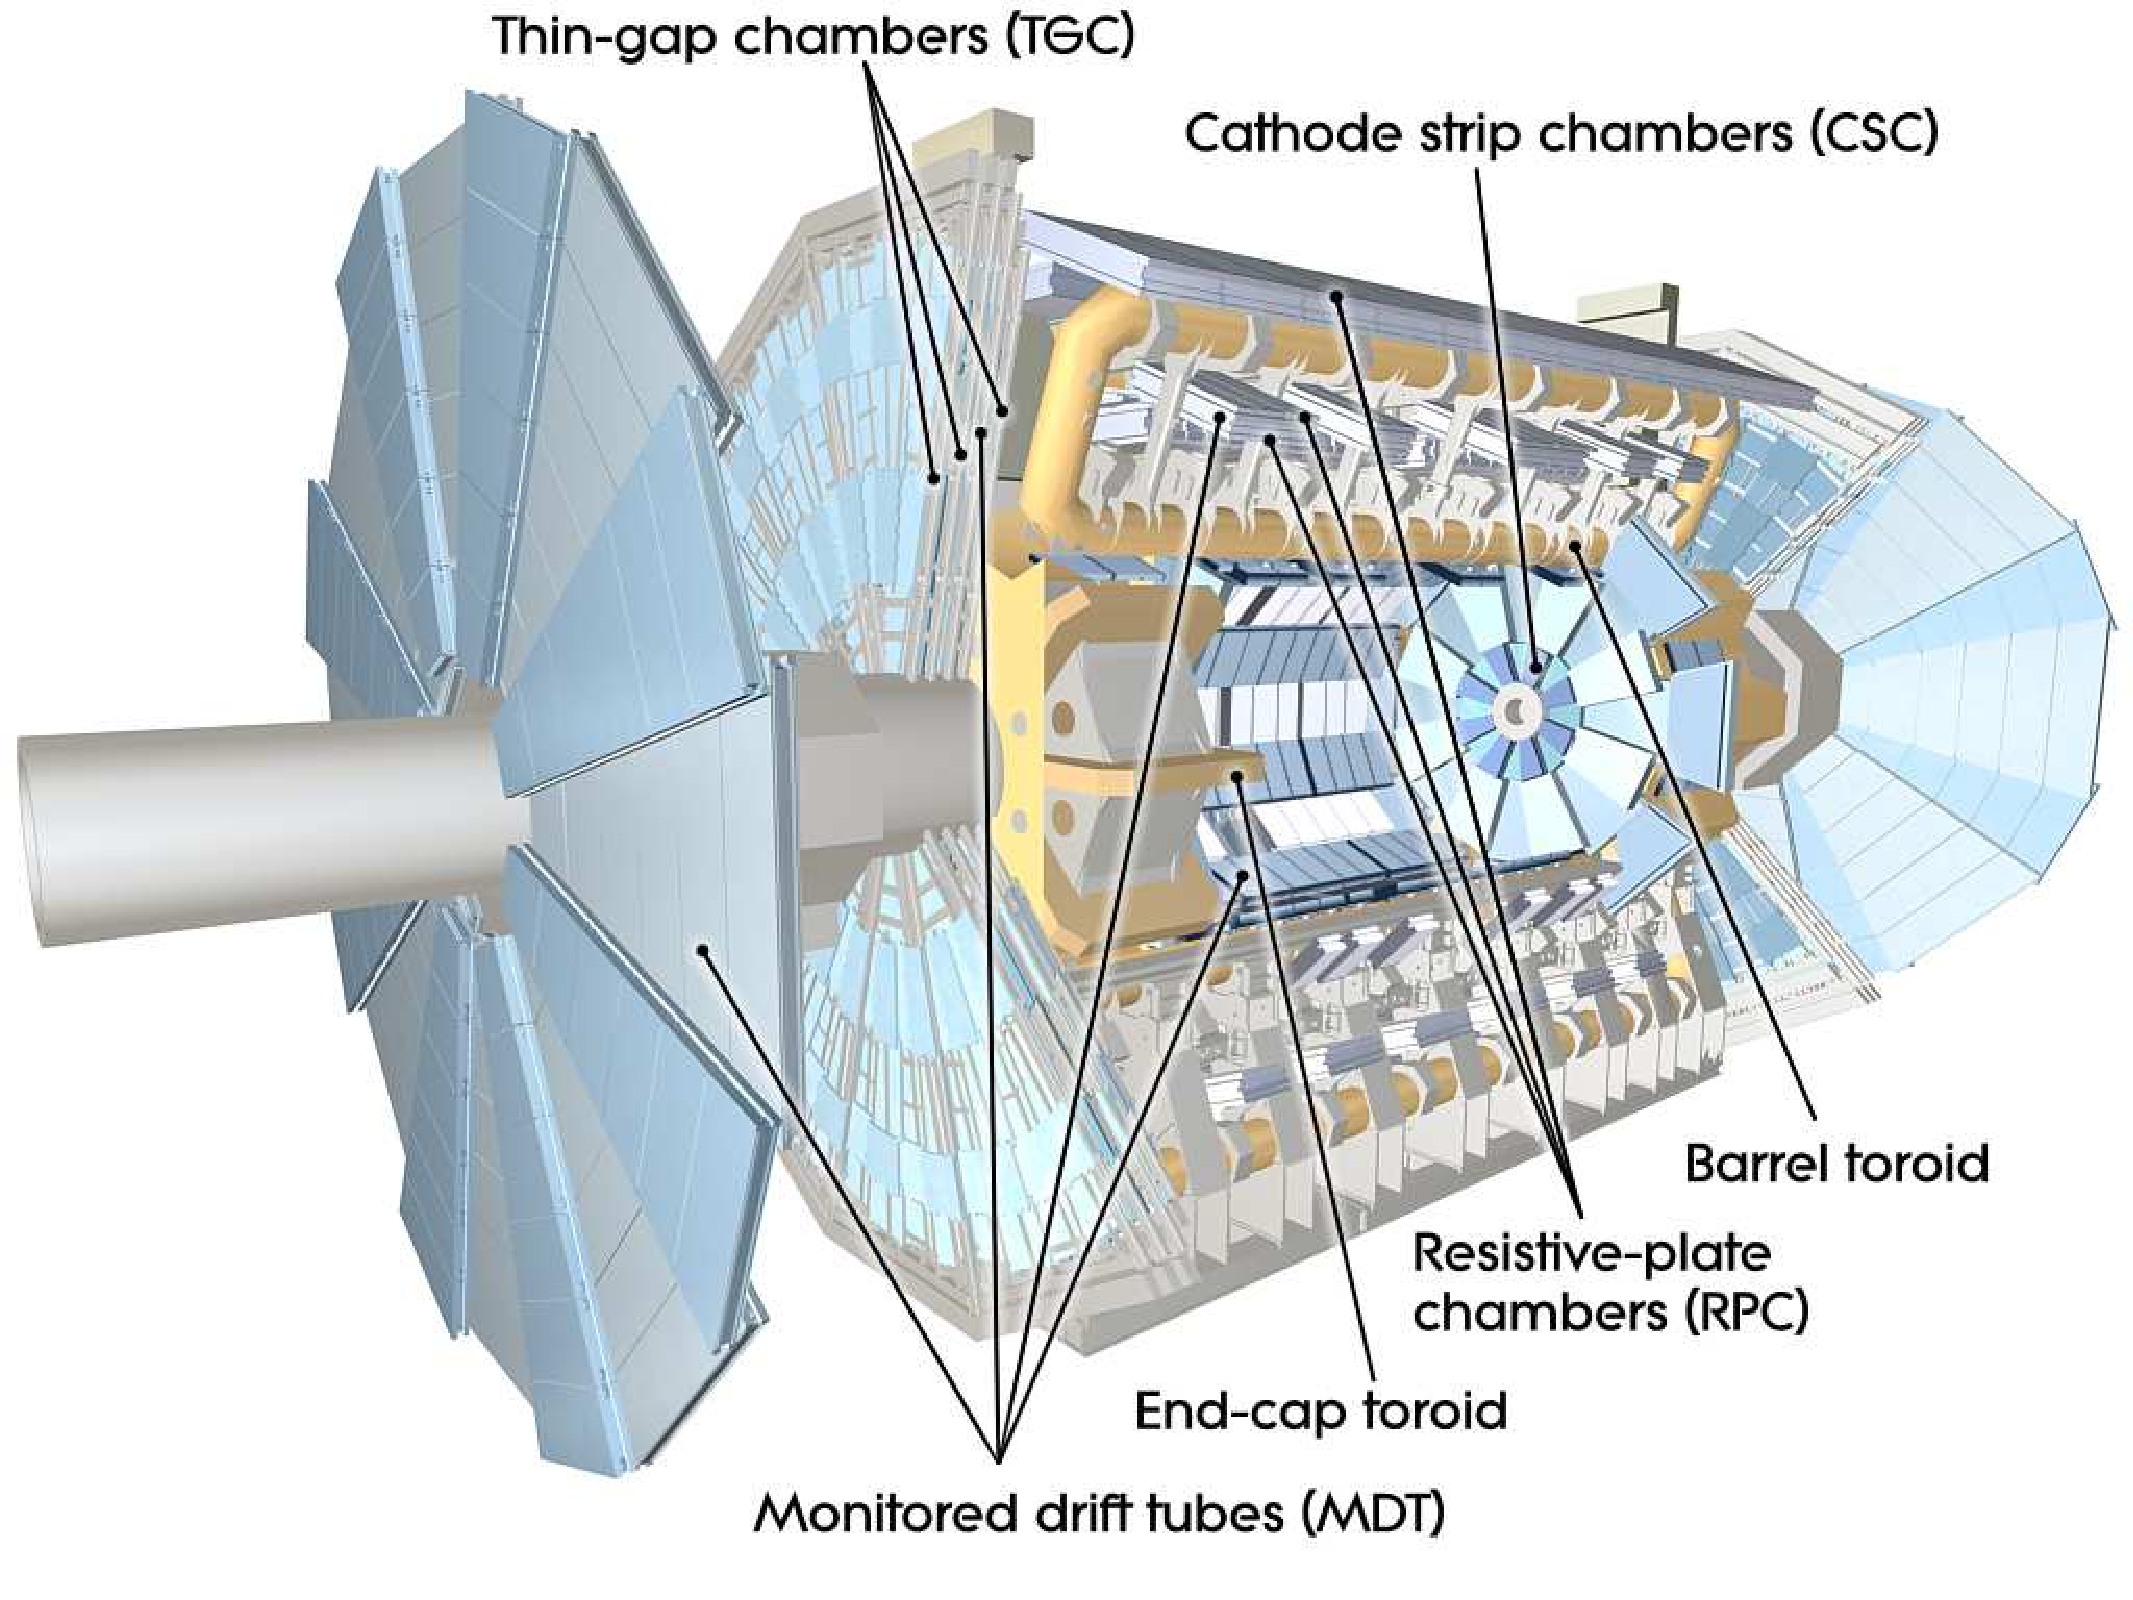
\includegraphics[width=0.8\linewidth]{figures/atlas/muon_system}
    \caption{ \cite{PERF-2007-01} A cut-away diagram of the ATLAS muon system
and its many sub-detectors.}
    \label{fig:muon_system}
  \end{center}
\end{figure}

Precision tracking measurements for momentum reconstruction is accomplished
using the Monitored Drift Tube chambers (MDTs) for $|\eta| < 2.0$ and using
Cathode-Strip Chambers (CSCs) for $2.0 < |\eta| < 2.7$.  The MDT system consists of
1163 drift tube chambers arranged in three to eight layers for varying $\eta$.
The CSCs are designed to withstand the higher rate and retain good time
resolution using multiwire proportional chambers with orthogonal segmented
cathode planes.

The MS also gives nanosecond tracking information for triggering on muon tracks.
This is accomplished using Resistive Plate Chambers (RPC) in the barrel region
$|\eta| < 1.05$ and Thin Gap Chambers (TGC) in the end-cap $1.05 < |\eta| < 2.4$
region.  Both chamber systems deliver a triggerable signal with a spread of
$15-25$ ns, thus providing the ability to tag individual beam-crossings.
